\documentclass{l4proj}

\usepackage{float}
\usepackage{amsmath}
\usepackage{subcaption} 


\begin{document}

%==============================================================================
%% METADATA
\title{Camera Controller}
\author{Dan Cristian Cecoi}
\date{22 February 2019}

\maketitle


\chapter{Background}

\section{Local Feature Detection}

Image local feature extraction is a dimensionality reduction technique where the resultant information provides a low dimensional description of the image contents. Local image features can be defined as a specific pattern that is unique to its immediately close pixels. These patterns are generally associated with a change of an image property or several properties simultaneously such as intensity, colour or texture. Local features are generally points but can be corners or blobs \citep{Tinne08}. These points serve as anchors whose neighbourhoods are represented by computed feature vectors. 

Local feature extraction is the most used low-level visual representation due to robustness to occlusion and clutter, their distinctiveness, repeatability and efficiency with achievable real-time performance. They can be used in applications such as image alignment, object recognition and motion tracking.   


\subsection{Scale Invariant Feature Transform}

A wide variety of feature description and detections algorithms have been proposed in literature. One of the most robust and scale-invariant feature detectors with high repeatability is Lowe's \textit{Scale Invariant Feature Transform} (SIFT). SIFT algorithm has four main steps:





\begin{enumerate}
  \item Scale Space Extrema Detection
  \item Key point Localization
  \item Orientation Assignment
  \item Description Generation 
\end{enumerate}





In order to identify interest points that are scale and orientation invariant, locations and scales that can be repeatably assigned under differing views of the same subject must be identified.  To achieve this, the scale space is separated into octaves and in each octave the initial image is repeatedly convolved with Gaussians to produce a set of scale space images. To find local extrema, each level of the pyramid has its adjacent Gaussians subtracted to produce a \textit{Difference of Gaussians} (DoG). 

To accurately locate interest points, key point candidates are localised and refined by using
a Taylor series expansion of the scale space to get a more accurate location of extrema. The
intensity at these extrema is compared to a contrast threshold value, and if its lower the
extrema is rejected. However, because the DoG function has a higher response along edges,
rejecting only key points with low contrast is not sufficient and the edge responses need to be removed as well. This is achieved by computing a 2x2 Hessian matrix, \textit{H}, at the location and scale of the keypoint, from which the principal curvature can be calculated. A poorly defined peak will have a large principal curvature across the edge but a small one in the
perpendicular direction. The eigenvalues of H are proportional to the principal curvatures of
the scale space function. Fortunately, it is not necessary to directly compute the eigenvalues
as we are only interested in the ratio between the largest magnitude eigenvalue and the
smaller magnitude eigenvalue. This ratio is compared with a threshold, \textit{r}, discarding the
keypoints whose ratio of principle curvatures is over that threshold \citep{Lowe04}.

\begin{figure}[ht]
    \centering
    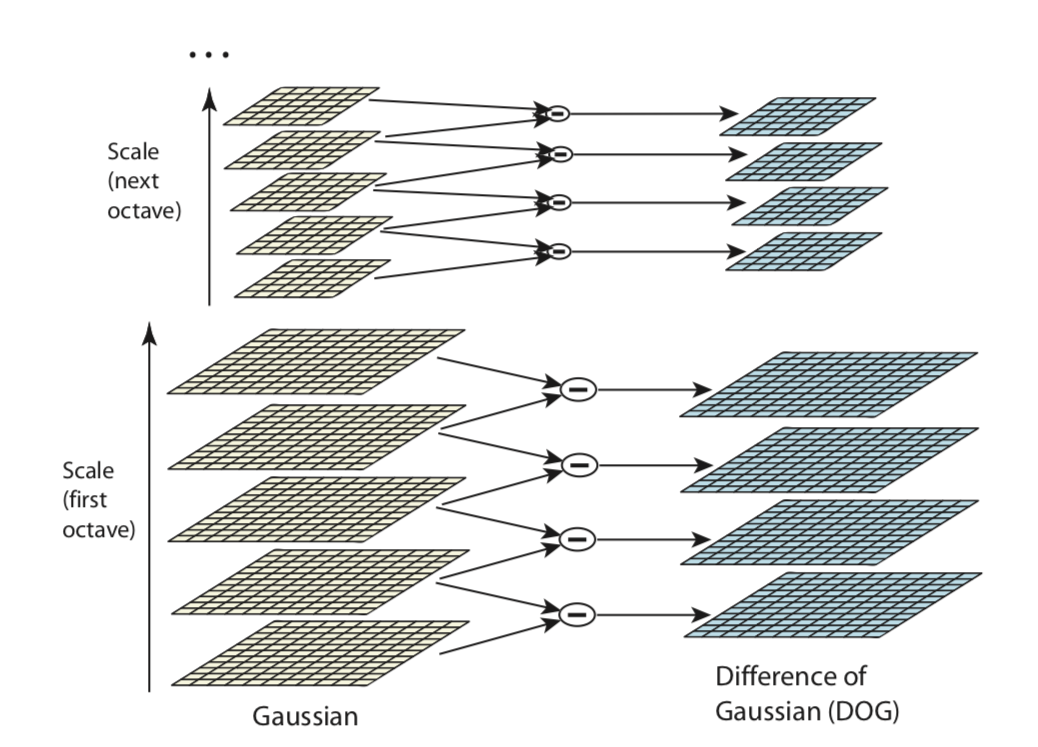
\includegraphics[width=0.8\textwidth]{l4template-master/images/gaussianPyramid.png}
    \caption{Each octave of the scale space is repeatedly convolved with Gaussians to produce the scale space images on the left. To produce the difference-of-Gaussian shown on the right, adjacent Gaussian images are subtracted. After each octave, the Gaussian image is down-sampled by a factor of 2, and the process repeated \citep{Lowe04}.}
    \label{gaussianpyramid}
\end{figure}

Orientation assignment is achieved by creating a orientation histogram of local gradient directions around the keypoint depending on the scale. The highest peak in the orientation histogram corresponds to the dominant direction of the key point.

\begin{figure}[ht]
    \centering
    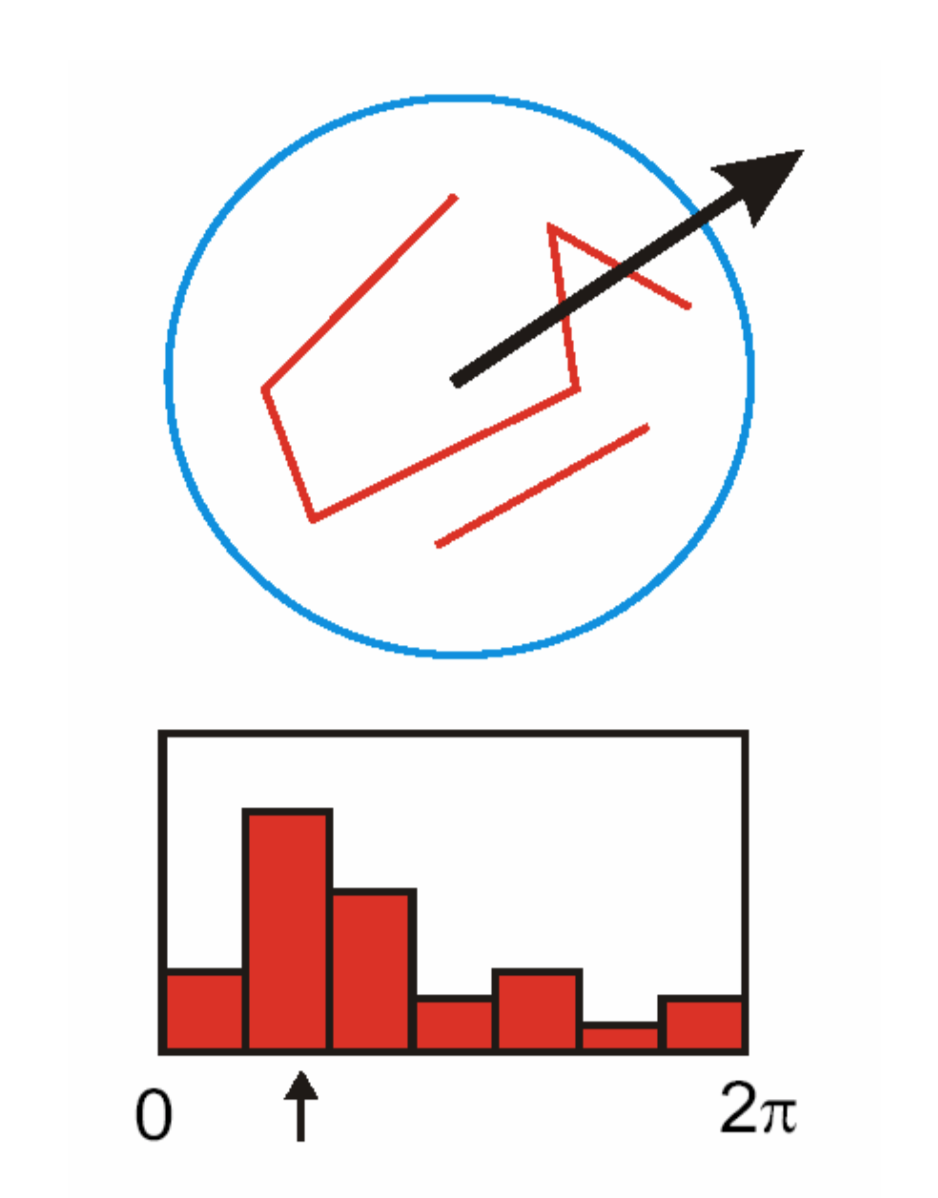
\includegraphics[width=0.3\textwidth]{l4template-master/images/orientationAssignment.png}
    \caption{Orientation Assignment by local gradient direction. \citep{Lowe04}}
    \label{orientationassignment}
\end{figure}

In the final step of the algorithm, the keypoint descriptor is created.  A 16-by-16 neighborhood around the keypoint is taken and subdivided into 4-by-4 sub regions. A orientation histogram is created over these sub regions by evaluating the magnitude of gradients in eight directions. All the orientation histograms are combined together into a 128 dimensional SIFT point descriptor. In addition to this, the feature vector is normalized in order to achieve robustness against illumination changes. 

\begin{figure}[ht]
    \centering
    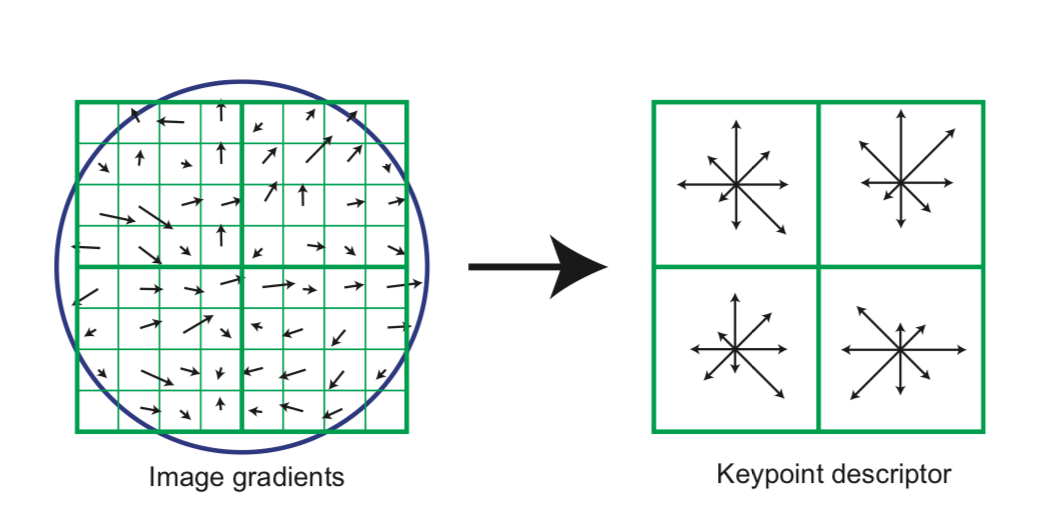
\includegraphics[width=0.7\textwidth]{l4template-master/images/keypointDescriptor.png}
    \caption{2x2 descriptor array computed from an 8x8 set of samples \citep{Lowe04}.}
    \label{keypointdescriptor}
\end{figure}


\subsection{Speeded Up Robust Features}

In the previous sub-section, SIFT algorithm for key point detection and description was described. While it became the most popular algorithm to extract distinctive invariant features from images, it was comparatively slow and a faster method was needed.

In 2006, Bay and Tuytelaars presented the Speeded Up Robust Features (SURF) algorithm that was partially inspired from SIFT, with similar steps but with different implementation details. 

To find points of interest, SURF uses a "Fast-Hessian" Detector which is based on the Hessian matrix due to its good performance in computation time and accuracy. Given a point p=(x,y) in an image, the Hessian Matrix \textit{H(p, $\sigma$)} at point \textit{p} and scale \textit{$\sigma$}, is: 

\begin{align}
 H(p,\sigma) = \begin{bmatrix}L_{xx}(p, \sigma) &L_{xy}(p, \sigma)  \\L_{yx}(p, \sigma) & L_{yy}(p, \sigma) \end{bmatrix}
\end{align}


Where $L_{xx}(p, \sigma)$ is the convolution of the Gaussian second order derivative with the image in point x. 

In SIFT, the approximation of Gaussian smoothing is achieved by using cascaded filters to detect scale-invariant characteristic points where the DoG is calculated on rescaled images. SURF pushes the approximation of the Laplacian of Gaussian even further and approximates it with box filters. These approximate second order Gaussian derivatives, and can be evaluated very efficiently using integral images, regardless of size, with the added benefit of removing the effects of aliasing when the images are sub-sampled \citep{Bay08}.





\begin{figure}[ht]
    \centering
    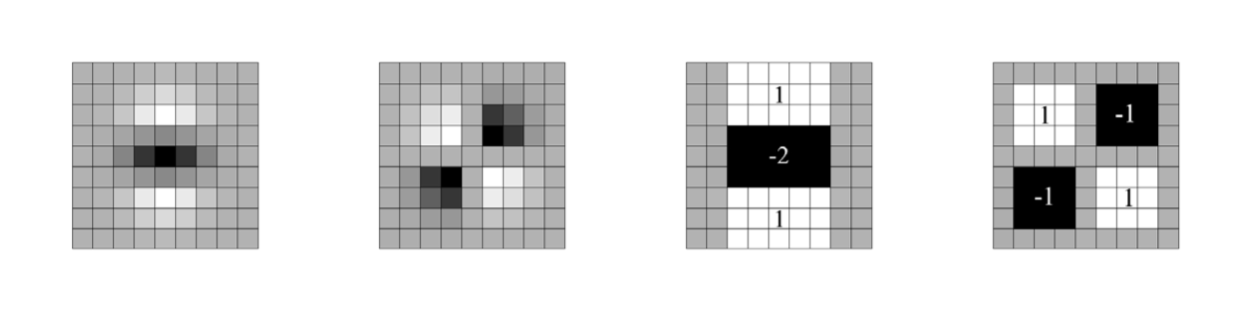
\includegraphics[width=0.7\textwidth]{l4template-master/images/boxfilters.png}
    \caption{The approximation of Gaussian second order partial derivatives using box filters \citep{Bay08}.}
    \label{boxfilters}
\end{figure}


Interest points at different scales are found by applying box filters of different sizes. The scale space is analyzed by up-scaling the filter size rather than iteratively reducing the image size. The following layers are obtained by filtering the image with gradually bigger masks, hence, for each new octave, the filter size increase is doubled. 

For the purpose of descriptor computation, the orientation of the point of interest must be determined. This is achieved by computing the Haar wavelet responses in horizontal and vertical directions around the point of interest. The dominant orientation is estimated by calculating a vector from the summation of all responses within a sliding orientation window covering a 60 degrees angle. Finally, the longest vector is selected which lends its orientation to the interest point. 

The descriptor is based on the sum of Haar wavelet responses. The region around the point is described by extracting a square region around the point of interest. The size of the region is directly proportional to the scale and is oriented along the orientation computed in the previous step. This region is split into smaller 4x4 square sub-regions and for each sub-region the Haar wavelet response is extracted. To offer more robustness for deformations, noise and translation the responses are weighted with a Gaussian. Finally, the responses are summed up over each sub-region to form a first set of entries to the feature vector. 

Bay et. all estimate that SURF outperforms SIFT by 4 times on average in computation time while not sacrificing in quality and robustness.

\section{Local Feature Matching}

\subsection{Matching strategies}
Matching descriptors from one set with the descriptors in a second set is usually performed by using two approaches: Brute Force Matching or applying a indexing structure. Brute Force Matcher is the simplest of the two. It functions by matching a descriptor from the first set with all the descriptors from the second set, returning the closest one based on the Euclidian distance \citep{Lowe04}. While this is not efficient, it is guaranteed to return the best matches of the two sets. 

For the purpose of achieving a better matching performance, an indexing structure is devised. One of the most widely used indexing structures are the k-d trees, which are a class of multi-dimensional search trees. This matching algorithm is much faster for larger data sets, however, it is not guaranteed to return the best match, as it only returns the approximate nearest neighbours. 

Outlier rejection from the feature space is accomplished by comparing the distance value of the closest match to the distance value of the second-closest match. In his seminal paper, Lowe suggests to reject all the matches with a distance ratio greater than 0.8, which was the approach used in this project. 

In order to further eliminate the remaining error matches, a robust estimation method introduced by \citet{Fischler81} called Random Sample Consensus (\textit{RANSAC}) is frequently used to to handle mapping features in the presence of outliers. 


\subsection{Homography}

Inlier correspondences between two images are found by computing the planar homography of the transformation. A homography, also known as plane projective transformation, is a 3 by 3 matrix \textit{H} that relates the transformation between corresponding image points as:
\begin{align}
x'=Hx 
\end{align}

Two images are related by a homography if and only if the image points correspond to the same planar surface in the real world and the images were acquired by rotating the camera about its optical axis. 

To compute the homography between two image pairs, RANSAC robust estimation is applied. For each iteration of the RANSAC algorithm:

\begin{enumerate}
    \item A random sample of 4 matches is selected and the homography \textit{H} is computed.
    \item The geometric image distance error for each match is calculated.
    \item The number of inliers from the number of matches for which the distance error is less than a threshold is computed.
    \item The homography with the largest number of inliers is selected.
    \item The least-squares homography estimate using all of the inliers is re-computed \citep{Torr2000}.
    
\end{enumerate}

 

%==================================================================================================================================
% \chapter{Implementation}
\chapter{Camera Controller}

\section{ONVIF Protocol}
One of the key requirements for the Camera Controller component was for it to be implemented in a non proprietary protocol not limited to a device. Because it is supported natively by the Pan Tilt Zoom (PTZ) Camera, and because it is by far the most popular open standard for the interface of physical IP-based security products, \textit{Open Network Video Interface Forum} (ONVIF) was chosen as the protocol in which this component will be implemented. ONVIF creates a standard for how IP Camera products within the security surveillance industry can communicate with each other. By using ONVIF, every IP security device can receive the same commands to execute some instruction such as to initiate video streaming or move a PTZ camera. Therefore, if in the future there is a decision to replace the camera with a different model that supports the ONVIF protocol, it wont be necessary to rewrite the base implementation of the Controller. 

On the most basic level, in the ONVIF protocol, the functions exposed to the client are defined in a Web Service Description Language (WSDL) file for each service and the commands are sent via Simple Object Access Protocol (SOAP) requests. A developer can choose to implement the functions based on the WSDL files and by following the ONVIF Core Specification. However, this project uses the \textbf{\textit{onvif-python}} library that offers an already implemented Access Point Interface (API) for these functions. This project is mostly using the ONVIF PTZ Service which defines the web service interface for configuration and operation of pan tilt zoom controllers. 

One of the big limitations of the ONVIF protocol is that for a camera to be considered ONVIF compliant only the "core" specification must be implemented by the manufacturer. In the Move Operations specification there are defined 3 different PTZ move operations: AbsoluteMove, RelativeMove and ContinuousMove. In AbsoluteMove the position argument of this command specifies the absolute position to which the PTZ unit moves. In RelativeMove the translation argument specifies the difference from the current position to the position to which the PTZ device is instructed to move. In ContinuousMove, the velocity argument of this command specifies a signed speed value for the Pan, Tilt and Zoom.  Even though AbsoluteMove and RelativeMove offer an increased granularity and sensitivity for the move operations,  ContinousMove was the only one to be implemented by the manufacturer of the PTZ Camera used in this project. 

In ContinousMove operation the PTZ command is executed continuously until a stop command is received by the camera. While this is perfectly adequate for applications such as controlling the camera from a joystick or by pressing buttons, it is not very suitable for the level of control required in this project. In order to move the camera a certain amount of degrees or pixels, the movement of the camera must be timed. 

In the prototyping phase, the velocity of the camera for Pan and Tilt was estimated by timing how much time it takes to complete a full rotation in each dimension. However, it soon became clear that there are significant errors caused by the network lag, the time the camera takes to process the commands and the inaccuracies caused by the PTZ motors not having a consistent velocity in each direction. 

To lessen the effect of these deficiencies, a predictive model that takes these variables into account needed to be developed.

\section{Controller Model}

With the aim of minimizing the effect of the limitation described in the previous sub-section, a Linear Regression model has been trained that will estimate a move time prediction taking into consideration the network delay, the signal lag and the physical inaccuracies of the camera. During the data gathering process it also soon became clear that the camera does not only move differently based on it being a pan or tilt movement, it also has a different behavior when it moves in different horizontal and vertical directions. Due to this observation, it was decided to train 4 different models depending on the movement that is required: Pan-Left, Pan-Right, Tilt-Up, Tilt-Down.  

\subsection{Data Gathering}

In order to train the Linear Regression model, it was necessary to gather data of the camera pixel displacement per unit time. To achieve this, PTZ Move requests were sent to the camera for a specific time interval. At each step of the data gathering process, the time interval was increased by 10 milliseconds. Data was collected for each of 4 pan-tilt directions, with an average of 2000 data points collected for each of them. 

To calculate the pixel displacement between two image pairs, a process based on a feature detector needed to be used. While the quality of the feature detection and matching was a vital characteristic in the search of a suitable algorithm, because the pixel displacement for over 8000 image pairs needed to be computed, the computational requirements also needed to be considered. SURF was selected over SIFT as the feature detector algorithm of choice for this task because of its decreased computation time with a similar quality of matches as SIFT. 

\begin{figure}[ht]
    \centering
    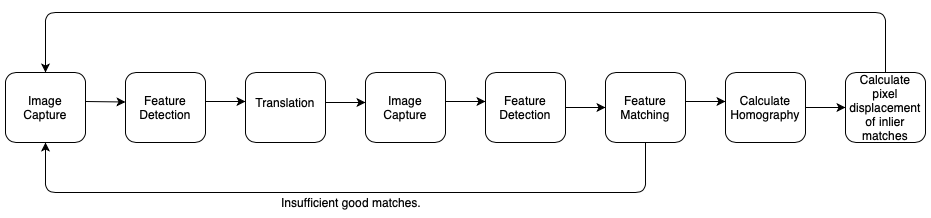
\includegraphics[width=1\textwidth]{l4template-master/images/dataGathering.png}
    \caption{Data Gathering Process}
    \label{datagathering}
\end{figure}


In the first part of the data gathering process, an image of an object is taken, and its features are detected using SURF. After the first set of features is computed, the camera translates for a specific amount of time and a second image is taken from which a second set of features is computed. To match the features between the two images, a choice needed to be made between the Brute Force Matcher (BFMatcher) and Fast Library for Approximate Nearest Neighbors (FLANN) based K-d tree algorithm. While FLANN has a lower computation time, the quality of the matches suffer as it is not guaranteed to produce the best matches. Because the quality of the matches was more important in this task than the increase in speed, BFMatcher was chosen as the matching algorithm. 

Once the potential matches were computed, the error matches were removed in a two part process. Firstly, a part of the error matches were removed by applying Lowe's ratio test described in the Background section. In the second part of the process, the homography of the transformation between the two images is computed using RANSAC and the outlier matches are rejected. 

Finally, the pixel displacement of every inlier match is computed and the median value is calculated in order to minimise the influence of any remaining outliers that were not rejected previously.  


\subsection{Model Training}

After analysing the plotting the collected data, it became apparent that there is a clear linear relationship between the camera translation time and the pixel displacement. Therefore, it was decided to train simple linear models for the Camera Controller. 

Firstly, a suitable choice for a framework capable of training a machine learning predictive model needed to be made. \textit{Scikit-learn} is a very powerful, open source library based on SciPy, NumPy, and matplotlib. While there are numerous others Machine Learning frameworks, such as TensorFlow, Keras, PyTorch, which are more suitable for more complex Machine Learning models than a linear regression, Scikit-learn was chosen for the familiarity, simplicity of use and the great built in support for different kinds of generalized linear models.

\begin{figure}[H]
  \begin{subfigure}[b]{0.5\textwidth}
    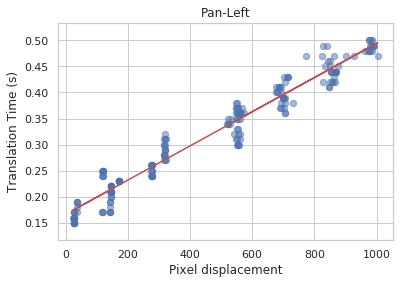
\includegraphics[width=\textwidth]{l4template-master/images/pan_left.png}
    \caption{Pan Left Model}
    \label{panleftmodel}
  \end{subfigure}
  %
  \begin{subfigure}[b]{0.5\textwidth}
    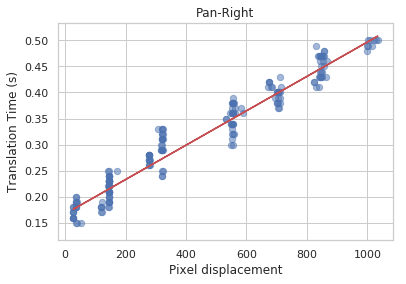
\includegraphics[width=\textwidth]{l4template-master/images/pan_right.png}
    \caption{Pan Right Model}
    \label{panrightmodel}
  \end{subfigure}
  \begin{subfigure}[b]{0.5\textwidth}
    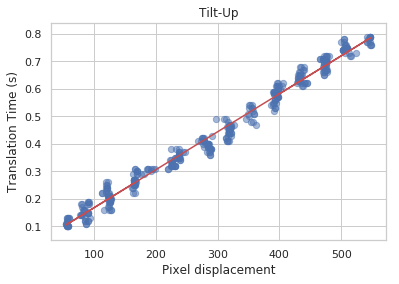
\includegraphics[width=\textwidth]{l4template-master/images/tilt_up.png}
    \caption{Tilt Up Model}
    \label{tiltup}
  \end{subfigure}
  \begin{subfigure}[b]{0.5\textwidth}
    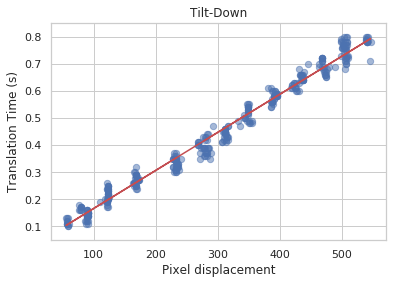
\includegraphics[width=\textwidth]{l4template-master/images/tilt_down.png}
    \caption{Tilt Down Model}
    \label{tiltdown}
  \end{subfigure}  
    
\end{figure}



Scikit-learn offers built in support for a big number of Linear Regression models, the most important of them being: Ordinary Least Squares, Lasso and Elastic Net. The later two are powerful techniques used for creating models in the presence of a very large number of features. The models apply regularisation techniques in order to penalise the magnitude of the less important features in the data set. Because the data used for training the models have only a feature per data point, the use of Lasso or Elastic Net was deemed unecessary and Ordinary Least Squares was used for training. 

Least Squares regression is the most common method for fitting a regression line. The underlying relationship between a dependent variable $y_{i}$ and an explanatory variable $x_{i}$ involving the error term $\epsilon_{i}$ can be described by:

\begin{align}
y = \alpha + \beta x_{i} + \epsilon _{i}
\end{align}


This method calculates the best-fitting line for the observed data by finding estimated values $ \hat{\alpha} $ and $\hat{\beta}$ which minimise the sum of the squares of the vertical deviations from each data point to the line. 

As part of the data preparation step, the outliers in the data were identified and removed by calculating the interquartile range (IQR) scores. IQR is is a measure of statistical dispersion, being equal to the difference between the upper and lower quartiles. While both variance and standard deviation are a measure of dispersion, IQR is much more robust to outliers. The data points that  were above 1.5 * IQR the 3rd quartile and below the 1st quartile were removed from the data. 

Based on the collected data, there was no translation for Pan and Tilt between the time intervals of 0.0 - 0.15 ms for Pan and 0.0 - 0.1 ms for tilt, therefore the data points corresponding to those time intervals were removed from the training set, resulting in better fitted models with a varience score of 0.95 for Pan models and 0.98 for Tilt models. 

The residual plots show that the difference between the predicted and real values are clustering around the lower y-axis digits. The data is also distributed on both sides of the y-axis, therefore the models don't tend to predict neither too low nor too high on average. However, one of the key requirements of a good residual plot is that there are no clear patterns on it. There is a clear quantisation of data both in the residual plots and in the Translation/Pixel displacement graphs. 

\begin{figure}[H]
  \begin{subfigure}[b]{0.5\textwidth}
    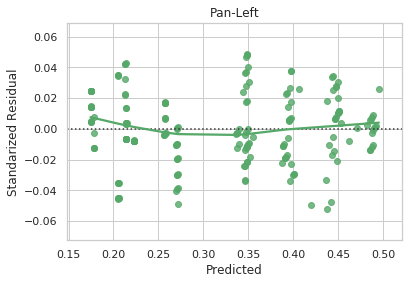
\includegraphics[width=\textwidth]{l4template-master/images/pan_left_residual.png}
    \caption{Pan Left Model Residual}
    \label{panleftmodelres}
  \end{subfigure}
  %
  \begin{subfigure}[b]{0.5\textwidth}
    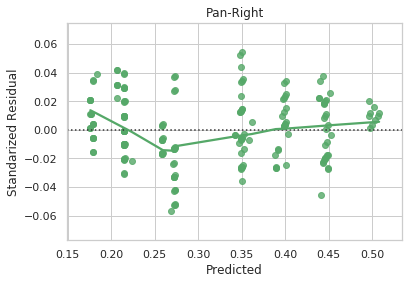
\includegraphics[width=\textwidth]{l4template-master/images/pan_right_residual.png}
    \caption{Pan Right Model Residual}
    \label{panrightmodelres}
  \end{subfigure}
  \begin{subfigure}[b]{0.5\textwidth}
    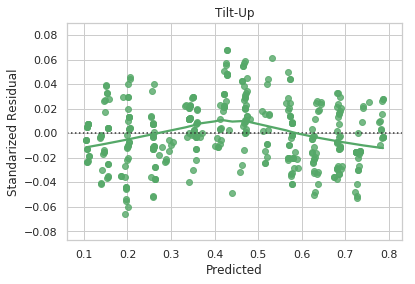
\includegraphics[width=\textwidth]{l4template-master/images/tilt_up_residual.png}
    \caption{Tilt Up Model Residual}
    \label{tiltupres}
  \end{subfigure}
  \begin{subfigure}[b]{0.5\textwidth}
    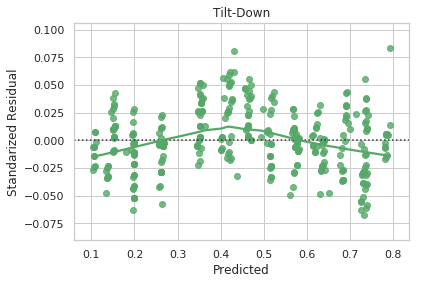
\includegraphics[width=\textwidth]{l4template-master/images/tilt_down_residual.png}
    \caption{Tilt Down Model}
    \label{tiltdownres}
  \end{subfigure}  
    
\end{figure}


To remove the possibility of errors in the matching process and the homography computation to be the underlying reasons for this grouping of data points, for a series of image pairs the pixel displacement was manually determined and compared with the pixel displacement computed using the data gathering process described above. The results were consistent, having an average error of less than 10 pixels. Hence, no deficiency in the data gathering process has been found and the physical characteristics of the camera were determined to be the reason for this phenomenon. 

Based on the collected data and the models, for a 1920 by 1080 pixels image, the smallest translation for pan is 37 pixels and 57 pixels for tilt.




\subsection{Controller Architecture}

After training a scikit-learn model, it is necessary to save the model for future use without having to retrain. This was achieved using Python's built-in persistence model called Pickle. Pickle is used for serializing and de-serializing Python object structures by converting a Python object hierarchies into byte streams that can be saved to files.


To direct the camera to a point on an object, the pixel coordinate on the image must be determined. Images in NumPy are multidimensional arrays, where each pixel value is stored as an element of the matrix that can be accessed by using NumPy's row-major-order indexing. Once the pixel coordinate has been selected, the Controller computes the direction and pixel distance of the point from image center. Depending on the direction, the suitable linear model is selected. The pixel displacement value is used as an input for that model with the output being the translation time prediction required for the camera to move in order to center on that specific point.

As mentioned above, the camera moves continuously from the moment a PTZ Command is received until the moment a Stop command is sent. This interval between the two commands is implemented using the built-in Python sleep() function used for pausing the execution of the program for a specific amount of time. Albeit this function is only accurate in the order of milliseconds and can be affected by the scheduling of other activities in the system and the implementation of the underlying Operating System's sleep function, it is perfectly acceptable for driving the camera with a similar expected performance across different Operating Systems.  



\begin{figure}[ht]
    \centering
    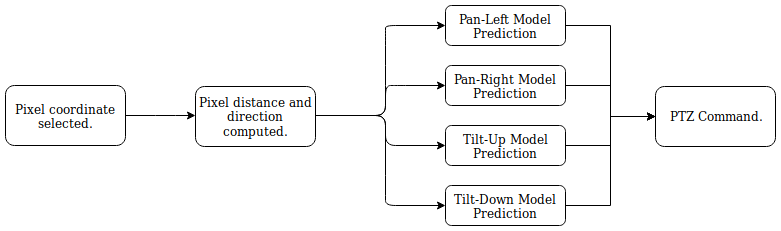
\includegraphics[width=1\textwidth]{l4template-master/images/Controller.png}
    \caption{Camera Controller}
    \label{controllerarchitecture}
\end{figure}


For the purpose of increasing the accuracy of the Camera movement, a simple retargeting algorithm was implemented. After a key point is selected and the camera translates to that point, local features are detected in the image after translation and the new position of the point is found. If the point is not found within the acceptable error margin from the image center, small incremental adjustments are performed using the smallest movement the camera is capable of until the point is within the acceptable distance. 



\subsection{Results}

 
[Paul, this is just for you to see the results, I will probably write this sub-chapter properly as part of the Validation chapter at the end. Will appreciate some guidance here about what I should write. ]
 
Once the models have been trained, the real-use case of the Camera Controller and the effectiveness of the Linear Regression models was tested. In order to get a good sample of key points with a good spread over the image, random key points were selected from the set. After the Camera movement finishes, the matching key point post translation is determined and the new distances are calculated. 

Using the retargeting algorithm improved the quality of translation drastically with a mean error of 9 pixels for tilt and 14 pixels for pan compared to 17 and 55 pixels respectively. This corresponds to approximately 1\% error.




\begin{figure}[H]
  \begin{subfigure}[b]{0.5\textwidth}
    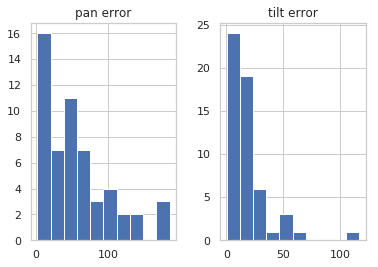
\includegraphics[width=\textwidth]{l4template-master/images/without.png}
    \caption{Error without retargeting.}
    \label{errorwithoutretargetting}
  \end{subfigure}
  %
  \begin{subfigure}[b]{0.5\textwidth}
    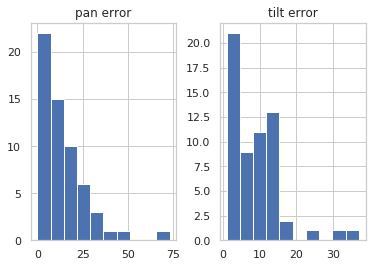
\includegraphics[width=\textwidth]{l4template-master/images/with_retargetting.png}
    \caption{Error with retargeting.}
    \label{errorwithretargetting}
  \end{subfigure}

    
\end{figure}

\bibliographystyle{abbrvnat}
\bibliography{l4proj}


\end{document}
